\documentclass[12pt] {article}

%%% Preambuła %%%
\usepackage[T1]{fontenc}
\usepackage[utf8]{inputenc}
\usepackage{polski}
\usepackage{lmodern}
\usepackage{hyperref}
\usepackage{mathptmx}
\usepackage{float}
\usepackage{graphicx}
\usepackage{amsmath}
\usepackage{listings}
\usepackage{booktabs}
\usepackage[table,xcdraw]{xcolor}


\usepackage{geometry}
\usepackage{pdflscape}

\geometry{a4paper, total={170mm,257mm}, left=20mm, top=20mm,}


\usepackage{forest}

\definecolor{folderbg}{RGB}{124,166,198}
\definecolor{folderborder}{RGB}{110,144,169}

\def\Size{4pt}
\tikzset{
      folder/.pic={
        \filldraw[draw=folderborder,top color=folderbg!50,bottom color=folderbg]
          (-1.05*\Size,0.2\Size+5pt) rectangle ++(.75*\Size,-0.2\Size-5pt);  
        \filldraw[draw=folderborder,top color=folderbg!50,bottom color=folderbg]
          (-1.15*\Size,-\Size) rectangle (1.15*\Size,\Size);
      }
    }

%%% Ustawienia listingów %%%
\definecolor{vgreen}{RGB}{104,180,104}
\definecolor{vblue}{RGB}{49,49,255}
\definecolor{vorange}{RGB}{255,143,102}

\lstdefinestyle{verilog-style}
{
    language=Verilog,
    basicstyle=\small\ttfamily,
    keywordstyle=\color{vblue},
    identifierstyle=\color{black},
    commentstyle=\color{vgreen},
	frame=single,
    tabsize=8,
    moredelim=*[s][\colorIndex]{[}{]},
    literate=*{:}{:}1
}

\makeatletter
\newcommand*\@lbracket{[}
\newcommand*\@rbracket{]}
\newcommand*\@colon{:}
\newcommand*\colorIndex{%
    \edef\@temp{\the\lst@token}%
    \ifx\@temp\@lbracket \color{black}%
    \else\ifx\@temp\@rbracket \color{black}%
    \else\ifx\@temp\@colon \color{black}%
    \else \color{vorange}%
    \fi\fi\fi
}
\makeatother


%%% Strona tytułowa %%%
\title {
	Języki Opisu Sprzętu \\
	\large Projekt: Elektroniczny Sejf Hotelowy \\
	Dokumentacja}

\author {
	Arkadiusz Kasprzak \\
	Jarosław Cierpich \\
	Wydział Fizyki i Informatyki Stosowanej \\ 
	Informatyka Stosowana}

	
\begin{document}

\begin{figure}
\centering

\includegraphics[scale = 1.5]{res/agh_znk_wbr_cmyk}
\end{figure}

%%% Strona tytułowa %%%
\maketitle

%%% Spis treści %%%
\newpage
\tableofcontents

\newpage
\section{Wstęp}
Niniejszy dokument stanowi dokumentację projektu \textbf{Elektroniczny Sejf Hotelowy} wykonanego w ramach przedmiotu \textbf{Języki Opisu Sprzętu} (WFiIS AGH) przez Jarosława Cierpicha i Arkadiusza Kasprzaka. Dokument ten zawiera m.in. założenia projektowe oraz opis wymaganej funkcjonalności, dokumentację przeznaczoną dla użytkownika projektu, dokumentację techniczną, analizę procesu syntezy oraz opis procedury testowania.

\section{Projekt}
Ten rozdział poświęcony został opisowi założeń projektowych oraz wymaganej funkcjonalności.

\subsection{Założenia projektowe}
Projekt dostarczać ma funkcji elektronicznego sejfu hotelowego, to znaczy pozwalać ma na otwieranie go za pomocą z góry ustalonego szyfru oraz późniejsze zamknięcie go. Projekt ma być zrealizowany na płytce rozwojowej \textbf{Zedboard} (do Xilinx Zynq-7000). Ze względu na okoliczności wykonywania projektu (projekt jako zaliczenie przedmiotu) przyjęte zostały pewne uproszczenia:
\begin{itemize}
\item czujnik zamknięcia sejfu zastąpiony zostaje przełącznikiem obsługiwanym przez użytkownika
\item szyfr jest parametrem projektu - nie jest możliwa jego modyfikacja na płytce bez powtórzenia procesu syntezy i implementacji
\item ruch rygla reprezentowany jest za pomocą dwóch diod LED dostępnych na płytce
\end{itemize}
Do realizacji projektu użyty ma być język \textbf{SystemVerilog} oraz środowisko \textbf{Xilinx Vivado}. 
Szyfr składać ma się z trzech liczb z przedziału \lbrack 0; 32). Liczby mają być wprowadzane przez użytkownika za pomocą pokrętła, przy czym kierunek obrotu pokrętła wskazuje, która liczba jest aktualnie wprowadzana: ruch zgody ze wskazówkami zegara oznacza pierwszą lub trzecią liczbę, ruch przeciwny do wskazówek zegara - drugą liczbę. Wprowadzenie nieprawidłowej liczby ma przerywać proces podawania szyfru - tzn. układ nie czeka, aż wprowadzony zostanie cały szyfr. Aktualnie wprowadzona liczba ma być prezentowana za pomocą wyświetlacza OLED.
Układ ma być w miarę możliwości pozbawiony błędów związanych z drganiami styków czy niestandardowym działaniem użytkownika.

\subsection{Wymagana funkcjonalność}
Od projektu wymaga się dostarczenia następującej funkcjonalności:
\begin{itemize}
\item możliwość wprowadzenia przez użytkownika poprawnego szyfru składającego się z trzech liczb z zakresu \lbrack 0; 32) za pomocą pokrętła
\item możliwość wprowadzenia przez użytkownika niepoprawnego szyfru, co automatycznie przerwać ma proces otwierania sejfu
\item możliwość monitorowania przez użytkownika aktualnego stanu otwarcia sejfu - za pomocą diod LED
\item możliwość monitorowania przez użytkownika aktualnie wprowadzanej wartości - za pomocą wyświetlacza OLED
\item możliwość rozpoczęcia procesu otwierania sejfu - za pomocą przycisku \textit{Open}
\item możliwość zamknięcia sejfu - za pomocą przycisku \textit{Close}
\item możliwość ustalenia aktualnej pozycji rygla sejfu - za pomocą przełącznika - zastępuje to czujnik zamknięcia sejfu
\item możliwość łatwego zaprogramowania nowego szyfru - zmiana trzech wartości w kodzie 
\end{itemize}



\newpage
\section{Dokumentacja użytkownika}
Rozdział przedstawia czynności, które należy wykonywać, aby poprawnie korzystać z urządzenia oraz oczekiwane działanie.

\subsection{Elementy wykorzystywane do interakcji z użytkownikiem}

\begin{figure}[H]
\centering
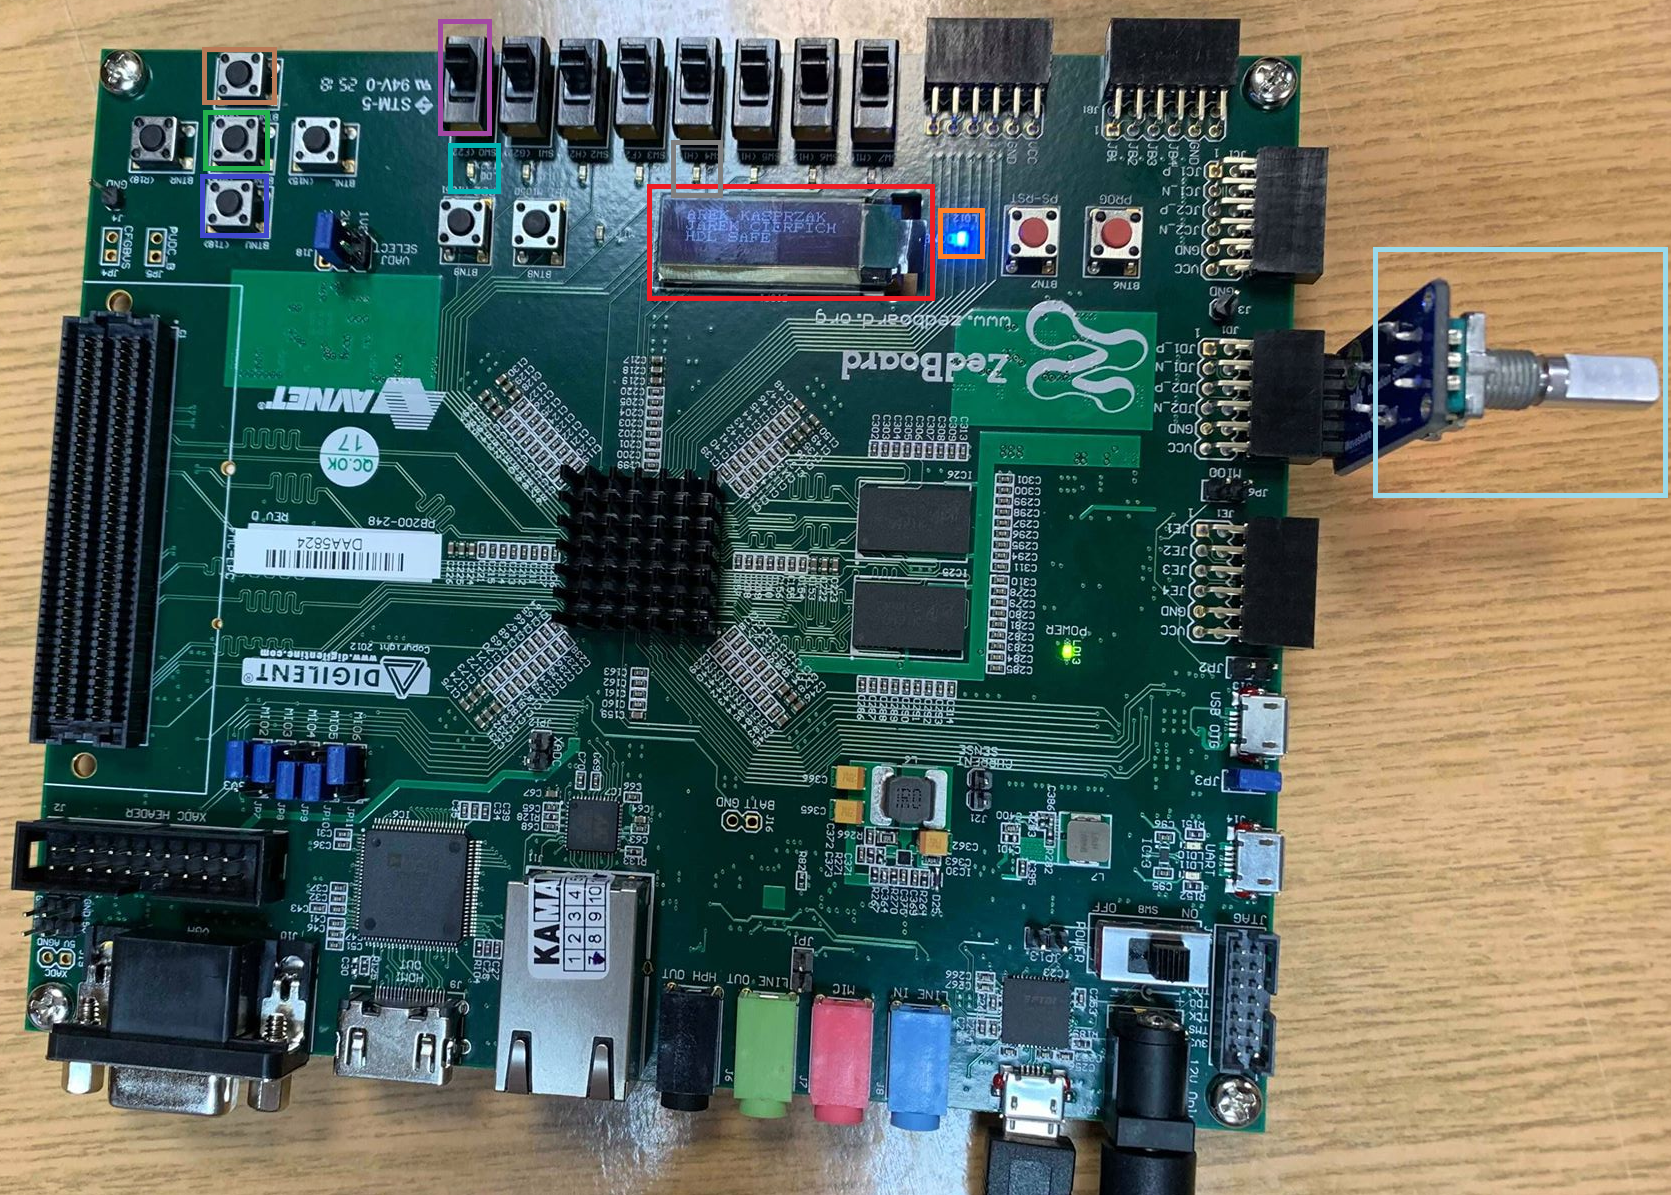
\includegraphics[width=1.0\textwidth]{res/user_doc/ui.png}
\caption{Elementy wykorzystywane do interakcji z użytkownikiem} 
\end{figure}

\begin{itemize}
\item kolorem \textcolor{red}{czerwonym} oznaczony został ekran OLED
\item kolorem \textcolor{blue}{niebieskim} oznaczony został przycisk rozpoczynający otwieranie sejfu
\item kolorem \textcolor{green}{zielonym} oznaczony został przycisk resetujący cały układ
\item kolorem \textcolor{brown}{brązowym} oznaczony został przycisk zamykający sejf
\item kolorem \textcolor{violet}{fioletowym} oznaczony został przełącznik odblokowujący funkcję zamykania sejfu
\item kolorem \textcolor{teal}{morskim} oznaczona została dioda sygnalizująca ruch rygla
\item kolorem \textcolor{orange}{pomarańczowym} oznaczona została dioda sygnalizująca gotowość układu do pracy, tj. wgranie oprogramowania na płytkę
\item kolorem \textcolor{darkgray}{ciemno szarym} oznaczona została dioda sygnalizująca otwarcie sejfu
\item kolorem \textcolor{cyan}{jasno-niebieskim} oznaczono pokrętło służące do wprowadzania kodu otwarcia
\end{itemize}

\newpage
\subsection{Korzystanie z urządzenia}
\begin{itemize}

\item Poprawne wgranie kodu na urządzenie można rozpoznać po zapalonej diodzie sygnalizującej  wgranie oprogramowania na płytkę oraz po napisie "Arek Kasprzak Jarek Cierpich HDL SAFE" na ekranie OLED

\item W przypadku niepoprawnego działania należy wykorzystać przycisk odpowiadający za reset

\item W celu rozpoczęcia otwierania należy wcisnąć przycisk do tego przeznaczony. Powodzenie akcji będzie można rozpoznać po zmianie napisu na ekranie OLED na: "CODE: 00". Napis ten wskazuje nam na aktualnie wprowadzoną część kodu, kod składa się z trzech dwucyfrowych liczb z zakresu od 0 do 32.

\newpage
\item Kod powinien zostać wprowadzony za pomocą pokrętła w następujący sposób:
\begin{itemize}
\item Pierwszą liczbę kodu należy wprowadzać przekręcając pokrętło zgodnie ze wskazówkami zegara. Wartość podawana na ekranie będzie się wtedy zwiększać.
\item Aby przejść do wybierania kolejnej części kodu należy zmienić kierunek kręcenia w momencie, gdy wybrana jest odpowiednia wartość (Jeżeli nasz kod składa się z liczby 9, 6 oraz 5, to zaczynamy kręcić w przeciwnym kierunku, gdy na ekranie znajduje się 9). Wartość podawana na ekranie będzie się wtedy zmniejszać.
\item Po osiągnięciu kolejnej części kodu (w podanym przykładzie 6) zaczynamy kręcić ponownie zgodnie ze wskazówkami zegara.
\item Przekręcamy pokrętło aż na ekranie będzie wyświetlana ostatnia część naszego kodu (w podanym przykładzie 5)
\item W przypadku niepowodzenia w wprowadzeniu kodu należy ponowić proces rozpoczęcia otwierania sejfu
\end{itemize}

\begin{figure}[H]
\centering
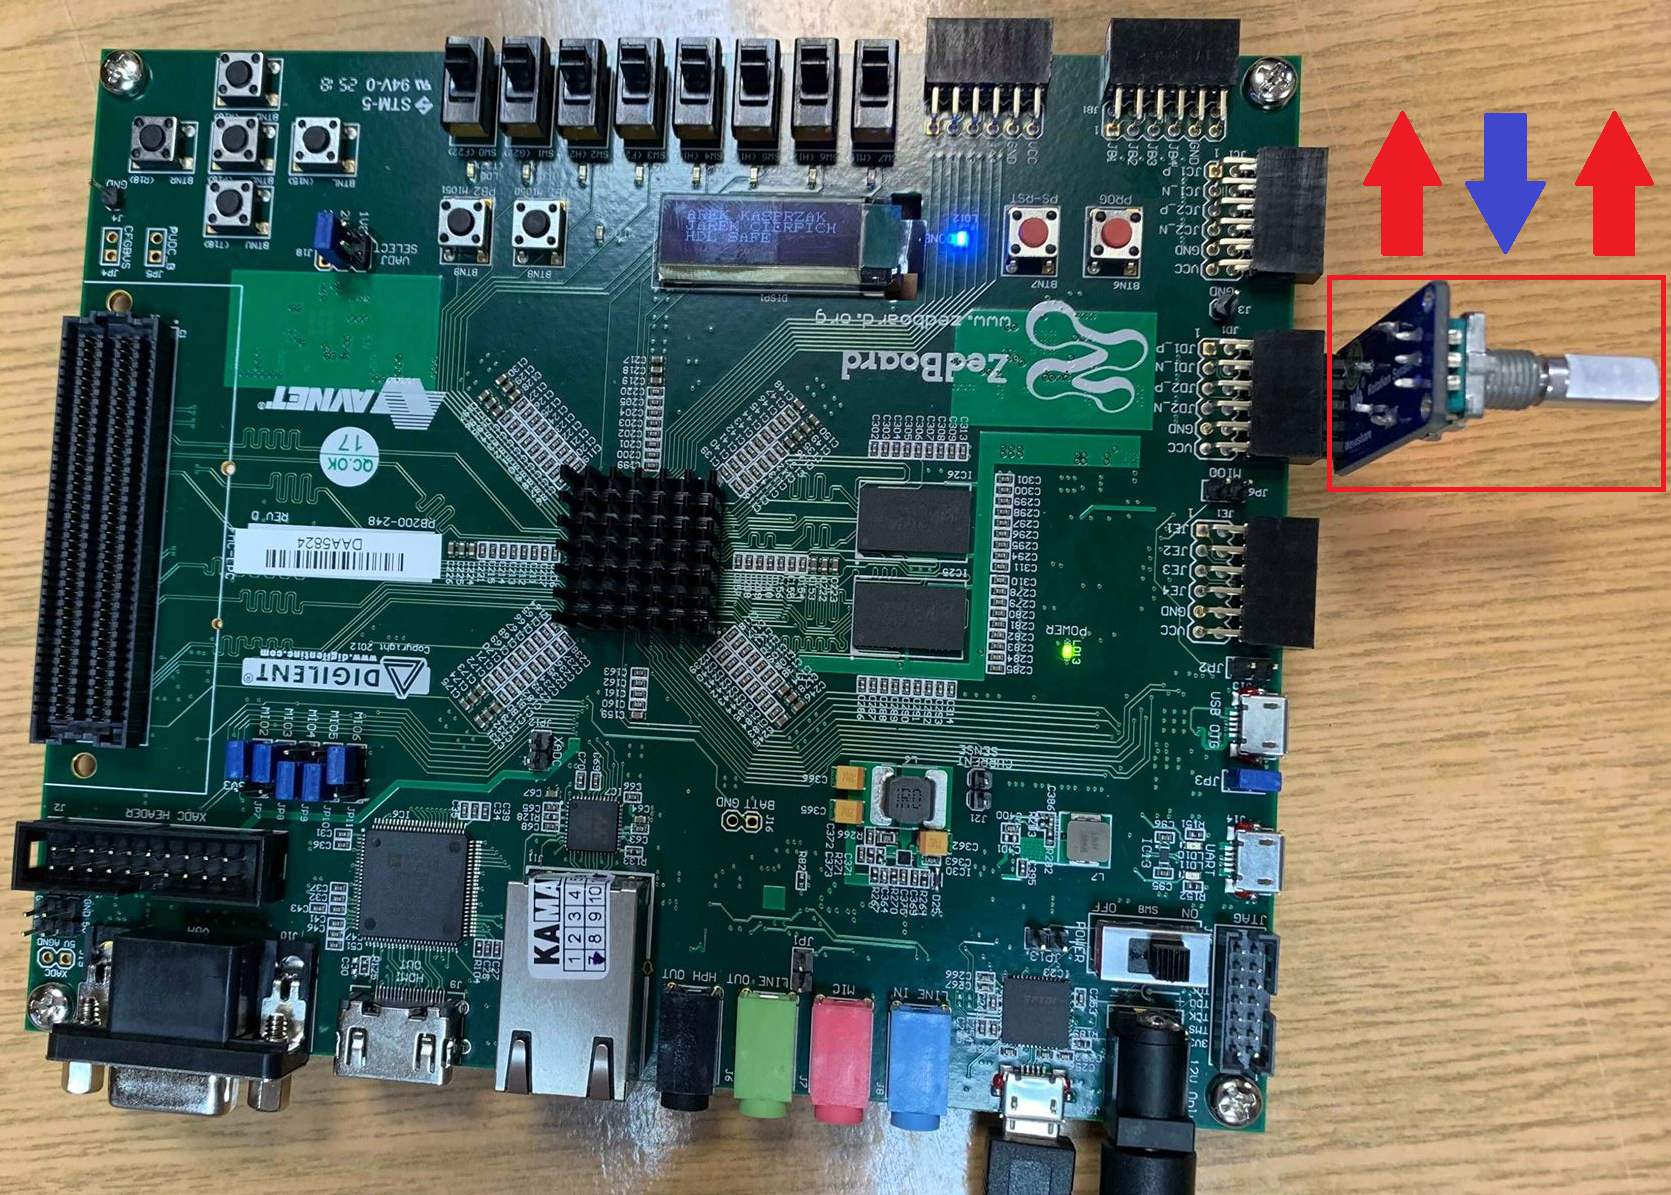
\includegraphics[width=1.0\textwidth]{res/user_doc/opening_knob.png}
\caption{Otwieranie sejfu} 
\end{figure}
\newpage

\item w przypadku wprowadzenia odpowiedniego kodu na chwilę zapali się dioda sygnalizująca ruch rygla oraz zapali się dioda sygnalizująca otwarcie sejfu

\item w celu ponownego zamknięcia sejfu należy przestawić przełącznik uruchamiający tą funkcję oraz kliknąć odpowiedni przycisk. Poprawne zamknięcie sejfu będzie widoczne poprzez zgaszenie się diody sygnalizującej otwarty sejf.

\begin{figure}[H]
\centering
\includegraphics[width=1.0\textwidth]{res/user_doc/how_to_close.png}
\caption{Zamykanie sejfu} 
\end{figure}
\newpage

\end{itemize}


\newpage
\section{Dokumentacja techniczna}
Rozdział opisuje szczegóły implementacji projektu - zarówno jeśli chodzi o warstwę sprzętową (hardware), jak i o oprogramowanie (software).

\subsection{Warstwa Hardware}
W tej sekcji zostanie przedstawiona architektura projektu z punktu widzenia \textbf{sprzętowego}


\begin{figure}[H]
\centering
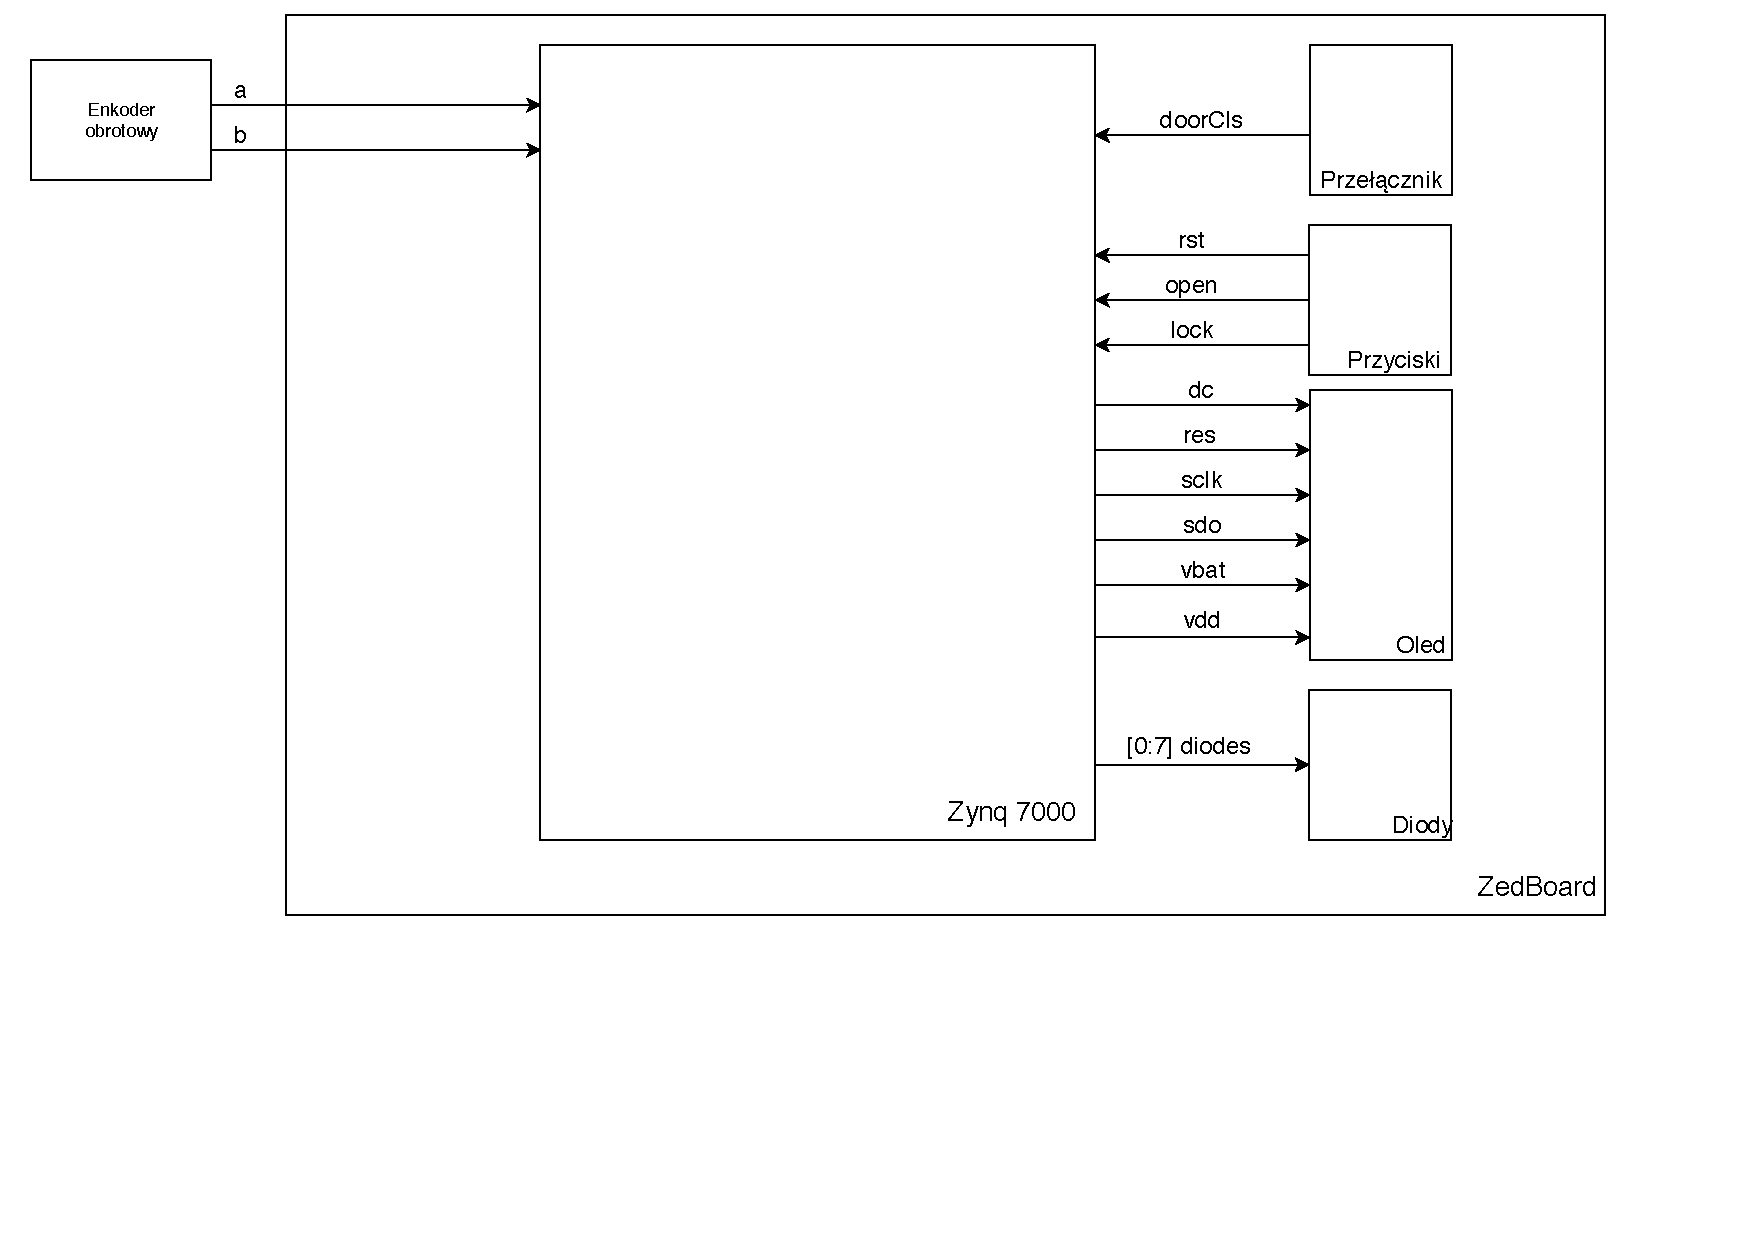
\includegraphics[width=1.1\textwidth]{res/hardware_architecture.pdf}
\caption{Przedstawia elementy sprzętowe użyte w projekcie oraz sygnały wymieniane między nimi.} 
\end{figure}
\label{fig:hwarch}
\newpage

Elementy użyte w realizacji projektu:
\begin{itemize}
\item \textbf{Enkoder obrotowy}, który za pomocą wysłanych sygnałów dostarcza informacji dotyczących obrotu oraz jego kierunku. Nie jest on częścią płytki Zynq 7000. Został podłączony za pomocą portów JD1\_N oraz JD2\_P
\item \textbf{FPGA} czyli programowalny układ logiczny. Steruje on całym układem. Element odpowiedzialny za logikę układu
\item \textbf{Przełącznik SW0} odpowiedzialny za dostarczanie sygnału odblokowania funkcji zamykania sejfu
\item \textbf{Przyciski BTNC, BTNU oraz BTND} odpowiedzialne za dostarczanie sygnałów zamykania, otwierania oraz resetowania układu
\item \textbf{Ekran OLED} który jest częścią płytki Zynq 7000. Wymaga on specjalnej procedury inicjalizującej. Informacje wysyłane są za pomocą protokołu SPI
\item \textbf{Diody}, służą do sygnalizowania informacji na temat ruchu rygla oraz stanu sejfu (zamknięty/otwarty) 
\end{itemize}

\newpage
\subsection{Warstwa Software - architektura}
W tej sekcji omówiona zostanie architektura projektu - zarówno ze względu na przepływ danych między komponentami, jak i na ich hierarchię w projekcie. \\
Rysunek \ref{fig:hier} przestawia hierarchię instancji modułów w projekcie, z wyróżnieniem instancji modułów odpowiedzialnych za tłumienie drgań na przyciskach i pokrętle - instancje te nie są generowane w czasie symulacji behawioralnej. \\
Rysunek \ref{fig:swarch} przedstawia strukturę zastosowanych w projekcie modułów wraz z przepływem danych między nimi. 

\begin{figure}[H]
\centering
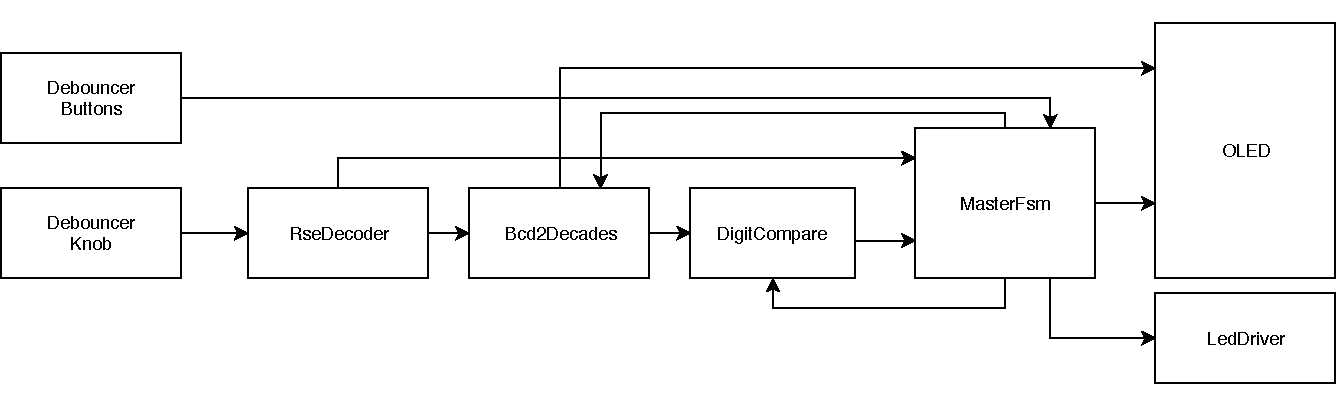
\includegraphics[width=1.0\textwidth]{res/architektura-moduly.pdf}
\caption{Struktura modułów oraz przepływ informacji} 
\label{fig:swarch}
\end{figure}

\begin{landscape}
\begin{figure}[H]
\centering
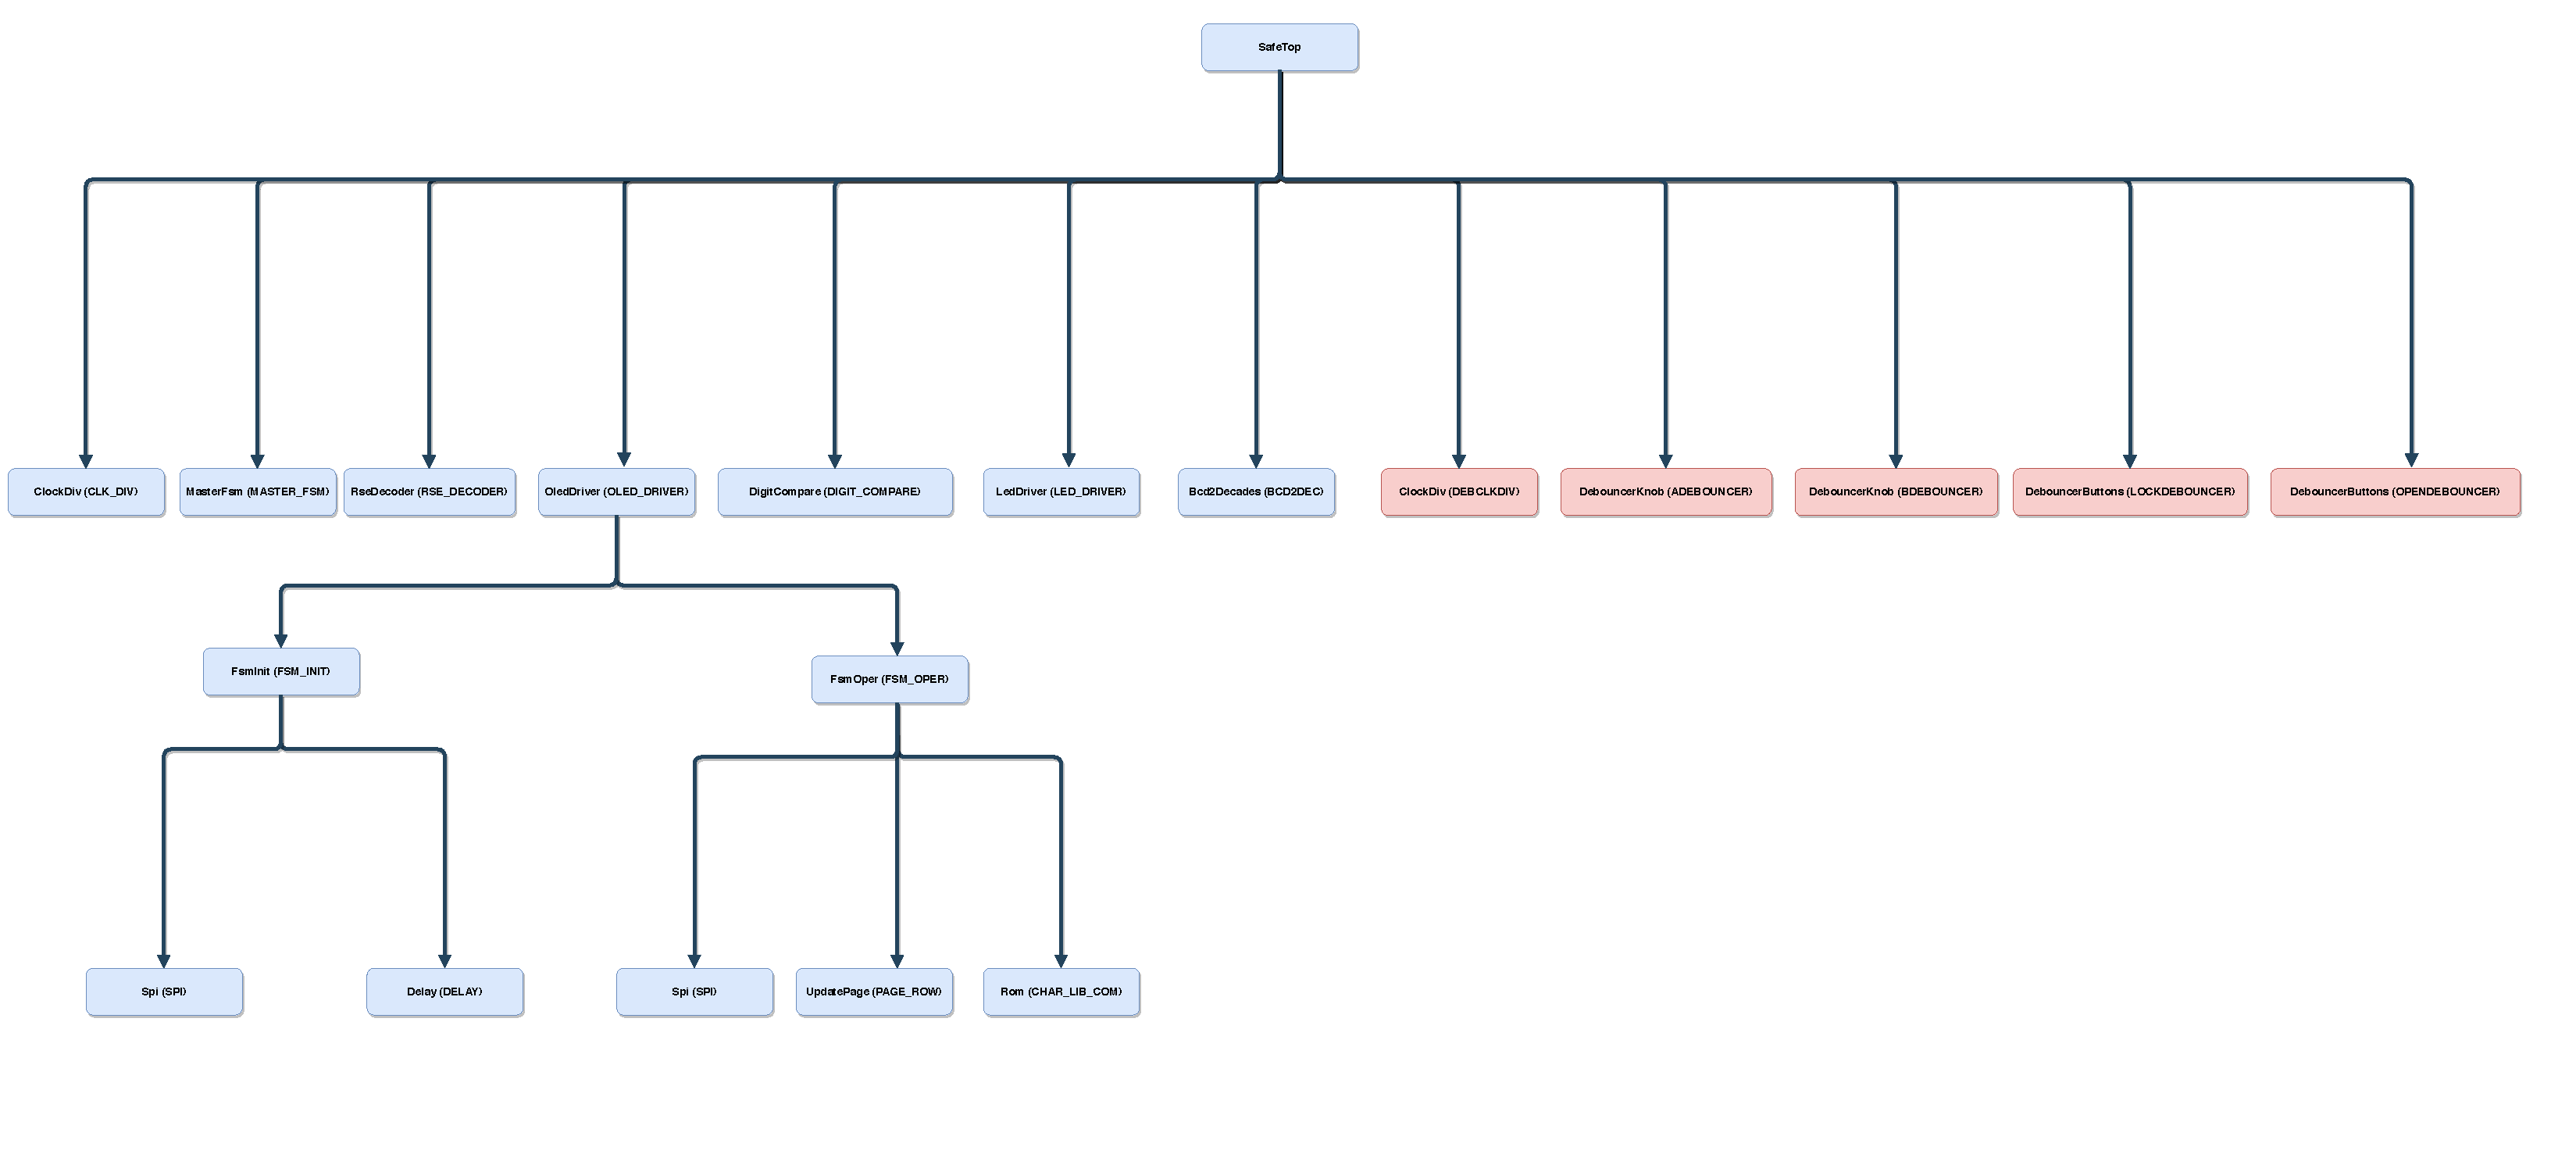
\includegraphics[width=1.5\textwidth]{res/HDL_Hierarchy.pdf}
\caption{Hierarchia instancji modułów zastosowana w projekcie. Nazwy w nawiasach to nazwy instancji, przed nawiasami - nazwy modułów. Na czerwono zaznaczono instancje, które nie są generowane podczas symulacji behawioralnej (wygaszanie drgań)} 
\label{fig:hier}
\end{figure}
\end{landscape}


\subsection{Warstwa Software - struktura projektu}
Wysokopoziomowa struktura katalogów i plików przedstawiona została poniżej:\\
\\
\begin{forest}
      for tree={
        font=\ttfamily,
        grow'=0,
        child anchor=west,
        parent anchor=south,
        anchor=west,
        calign=first,
        inner xsep=7pt,
        edge path={
          \noexpand\path [draw, \forestoption{edge}]
          (!u.south west) +(7.5pt,0) |- (.child anchor) pic {folder} \forestoption{edge label};
        },
        % style for your file node 
        file/.style={edge path={\noexpand\path [draw, \forestoption{edge}]
          (!u.south west) +(7.5pt,0) |- (.child anchor) \forestoption{edge label};},
          inner xsep=2pt,font=\small\ttfamily
                     },
        before typesetting nodes={
          if n=1
            {insert before={[,phantom]}}
            {}
        },
        fit=band,
        before computing xy={l=15pt},
      }  
		[TopSafe
			[TopSafe.xpr,file]
			[TopSafe.srcs
				[constrs\_1]
				[sim\_1]
				[sources\_1]
      		]
      	]	
\end{forest} \\
\\
Jest to standardowy podział dla narzędzia \textbf{Xilinx Vivado}. Plik \textbf{TopSafe.xpr} jest głównym plikiem projektu. Struktura wewnętrzna katalogu \textbf{constrs\_1} jest następująca: \\ 
\\
\begin{forest}
      for tree={
        font=\ttfamily,
        grow'=0,
        child anchor=west,
        parent anchor=south,
        anchor=west,
        calign=first,
        inner xsep=7pt,
        edge path={
          \noexpand\path [draw, \forestoption{edge}]
          (!u.south west) +(7.5pt,0) |- (.child anchor) pic {folder} \forestoption{edge label};
        },
        % style for your file node 
        file/.style={edge path={\noexpand\path [draw, \forestoption{edge}]
          (!u.south west) +(7.5pt,0) |- (.child anchor) \forestoption{edge label};},
          inner xsep=2pt,font=\small\ttfamily
                     },
        before typesetting nodes={
          if n=1
            {insert before={[,phantom]}}
            {}
        },
        fit=band,
        before computing xy={l=15pt},
      }  
		[constrs\_1
			[new
				[constraints.xdc,file]
      		]
      	]	
\end{forest} \\
\\
Zawiera on plik \textit{.xdc} z tzw. Design Constraints. Katalog \textbf{sim\_1} zawiera moduły testujące (tzw. Testbench) i jego strukturę przedstawiono poniżej: \\
\\
\begin{forest}
      for tree={font=\ttfamily, grow'=0, child anchor=west, parent anchor=south, anchor=west, calign=first, inner xsep=7pt,
        edge path={ \noexpand\path [draw, \forestoption{edge}] (!u.south west) +(7.5pt,0) |- (.child anchor) pic {folder} \forestoption{edge label}; },
        % style for your file node 
        file/.style={edge path={\noexpand\path [draw, \forestoption{edge}]
          (!u.south west) +(7.5pt,0) |- (.child anchor) \forestoption{edge label};}, inner xsep=2pt,font=\small\ttfamily },
        before typesetting nodes={if n=1 {insert before={[,phantom]}} {} }, fit=band, before computing xy={l=15pt}, }  
		[sim\_1
      		[new
      			[OLED
      				[TbOledDriver.sv,file]
      			]
				[TbBcd2Decades.sv,file]
				[TbClkDiv.sv,file]
				[TbDebouncerButtons.sv,file]
				[TbDelay.sv,file]
				[TbDigitCompare.sv,file]
				[TbLedDriver.sv,file]
				[TbMasterFsm.sv,file]
				[TbRseDecoder.v,file]
				[TbSafeTop.sv,file]
			]
		]
\end{forest} \\
\\ \\ \\ \\ \\
Struktura katalogu \textbf{sources\_1} zawierającego kod źródłowy projektu: \\	
\\	
\begin{forest}
      for tree={ font=\ttfamily, grow'=0, child anchor=west, parent anchor=south, anchor=west, calign=first, inner xsep=7pt,
        edge path={\noexpand\path [draw, \forestoption{edge}] (!u.south west) +(7.5pt,0) |- (.child anchor) pic {folder} \forestoption{edge label}; },
        % style for your file node 
        file/.style={edge path={\noexpand\path [draw, \forestoption{edge}] (!u.south west) +(7.5pt,0) |- (.child anchor) \forestoption{edge label};}, inner xsep=2pt,font=\small\ttfamily },
        before typesetting nodes={if n=1 {insert before={[,phantom]}} {} },
        fit=band, before computing xy={l=15pt}, }  
		[sources\_1
			[new
				[Bcd2Decades.sv,file]
				[ClockDiv.sv,file]
				[DebouncerButtons.sv,file]
				[DebouncerKnob.v,file]
				[DigitCompare.sv,file]
				[LedDriver.sv,file]
				[MasterFsm.sv,file]
				[safeTop.sv,file]
				[RseDecoder.sv,file]
				[OLED
					[delay.sv,file]
					[fsm\_init.sv,file]
					[fsm\_oper.sv,file]
					[OledDriver.sv,file]
					[pixel\_SSD1306.dat,file]
					[rom.v,file]
					[screens.vh,file]
					[spi.sv,file]
					[update\_page.sv,file]
				]	
			]
		]
\end{forest}


\subsection{Warstwa Software - parametry i moduły projektu}
Ten podrozdział opisuje część implementacji projektu - zastosowane parametry oraz moduły napisane w języku SystemVerilog.

\subsubsection{Parametry projektu}
Główny moduł projektu udostępnia następujące \textbf{parametry} pozwalające na modyfikację działania sejfu:
\begin{itemize}
\item \textbf{slowClockPeriodLength} - współczynnik oznaczający wartość dzielnika częstotliwości zegara, którym taktowany jest sejf (z wyjątkiem debouncerów i wyświetlacza OLED). Wartość domyślna: 100000.
\item \textbf{debouncerClockPeriodLength} - współczynnik oznaczający wartość dzielnika częstotliwości zegara, którym taktowane są debouncery w projekcie. Wartość domyślna: 300007.
\item \textbf{areDebouncersUsed} - flaga włączająca lub wyłączająca generację debouncerów w projekcie. Wartość domyślna: 1 - debouncery mają zostać wygenerowane.
\item \textbf{firstCodeNumber} - pierwsza liczba szyfru. Wartość domyślna: 15.
\item \textbf{secondCodeNumber} - druga liczba szyfru. Wartość domyślna: 30.
\item \textbf{thirdCodeNumber} - trzecia liczba szyfru. Wartość domyślna: 9.
\end{itemize}

\subsubsection{Lista modułów projektu}
Projekt składa się z następujących \textbf{modułów}:
\begin{itemize}
\item \textbf{SafeTop} - główny moduł projektu
\item \textbf{Bcd2Decades} - licznik BCD (Binary Coded Decimal) o dwóch dekadach
\item \textbf{ClockDiv} - dzielnik zegara
\item \textbf{DebouncerButtons} - układ wygaszający drgania na przyciskach
\item \textbf{DebouncerKnob} - układ wygaszający drgania na pokrętle
\item \textbf{DigitCompare} - układ porównujący wprowadzone przez użytkownika liczby z szyfrem 
\item \textbf{LedDriver} - sterownik diod LED
\item \textbf{MasterFsm} - główna logika sejfu
\item \textbf{RseDecoder} - układ odpowiedzialny za komunikację z pokrętłem
\item Moduły odpowiedzialne za \textbf{obsługę wyświetlacza OLED}: 
\begin{itemize}
\item \textbf{OledDriver} - główny moduł odpowiedzialny za obsługę wyświetlacza
\item \textbf{Delay} - moduł odpowiedzialny za generowanie opóźnień
\item \textbf{FsmInit} - moduł odpowiedzialny za przeprowadzenie procedury inicjalizacji wyświetlacza OLED
\item \textbf{FsmOper} - moduł odpowiedzialny za wysyłanie danych do wyświetlacza OLED
\item \textbf{Rom} - transkoder działający na zasadzie pamięci stałej - odpowiada za dostarczenie \textit{czcionki}
\item \textbf{Spi} - implementacja uproszczonego (jednokierunkowego) protokołu SPI
\item \textbf{UpdatePage} - moduł powiązany z FsmOper
\end{itemize}
\end{itemize}
Do implementacji modułów obsługujących wyświetlacz OLED wykorzystany został w dużej części kod przygotowany w ramach zajęć laboratoryjnych z przedmiotu Języki Opisu Sprzętu. Dalsza część dokumentacji zawiera opis działania najważniejszych modułów projektu.

\subsubsection{Moduł SafeTop}
Jest to moduł usytuowany najwyżej w hierarchii projektu - odpowiedzialny jest on za połączenie ze sobą pozostałych modułów w projekcie za pomocą ich sygnałów wejściowych i wyjściowych. Ponadto zawiera on logikę odpowiedzialną za generowanie instancji debouncerów tylko, gdy do modułu przekazany zostanie parametr \textbf{areDebouncersUsed} o wartości 1 (logiczna prawda). Zostało to osiągnięte za pomocą \textbf{bloku generate} połączonego z instrukcją sterującą if-else. Listing \ref{lst:generate} przestawia implementację opisywanego rozwiązania. Schemat blokowy przedstawiony na rysunku \ref{fig:deb} ilustruje ideę zastosowanego algorytmu.
\begin{lstlisting}[style={verilog-style}, caption={Przykład zastosowania bloku generate do warunkowego generowania instancji debouncerów w module SafeTop}, label={lst:generate}]
generate 
    if (areDebouncersUsed) begin : debGen
        
        // clock divider for debouncers
        wire debSlowClk;
       	ClockDiv #(.clockPeriodLength(debouncerClockPeriodLength))
       	DEBCLKDIV 
       	(
       	    .clk(clk), .rst(rst), 
            .slowClk(debSlowClk)
        );
            
        // a signal debouncer 
        DebouncerKnob #(.N(3)) ADEBOUNCER (
            .clk(debSlowClk), .rst(rst), .in(a), .out(aKnob)
        );
            
        // b signal debouncer 
        DebouncerKnob #(.N(3)) BDEBOUNCER (
            .clk(debSlowClk), .rst(rst), .in(b), .out(bKnob)
        );
            
        // open signal debouncer
        DebouncerButtons #(.registerSize(3)) OPENDEBOUNCER (
            .clk(debSlowClk), .rst(rst), .in(open), .out(openDeb)
        );
            
        // lock signal debouncer
        DebouncerButtons #(.registerSize(3)) LOCKDEBOUNCER (
            .clk(debSlowClk), .rst(rst), .in(lock), .out(lockDeb)
        );
            
    end
    else begin : debNoGen
    	assign aKnob = a;
        assign bKnob = b;
        assign openDeb = open;
        assign lockDeb = lock;
    end
endgenerate
\end{lstlisting}

\begin{figure}[H]
\centering
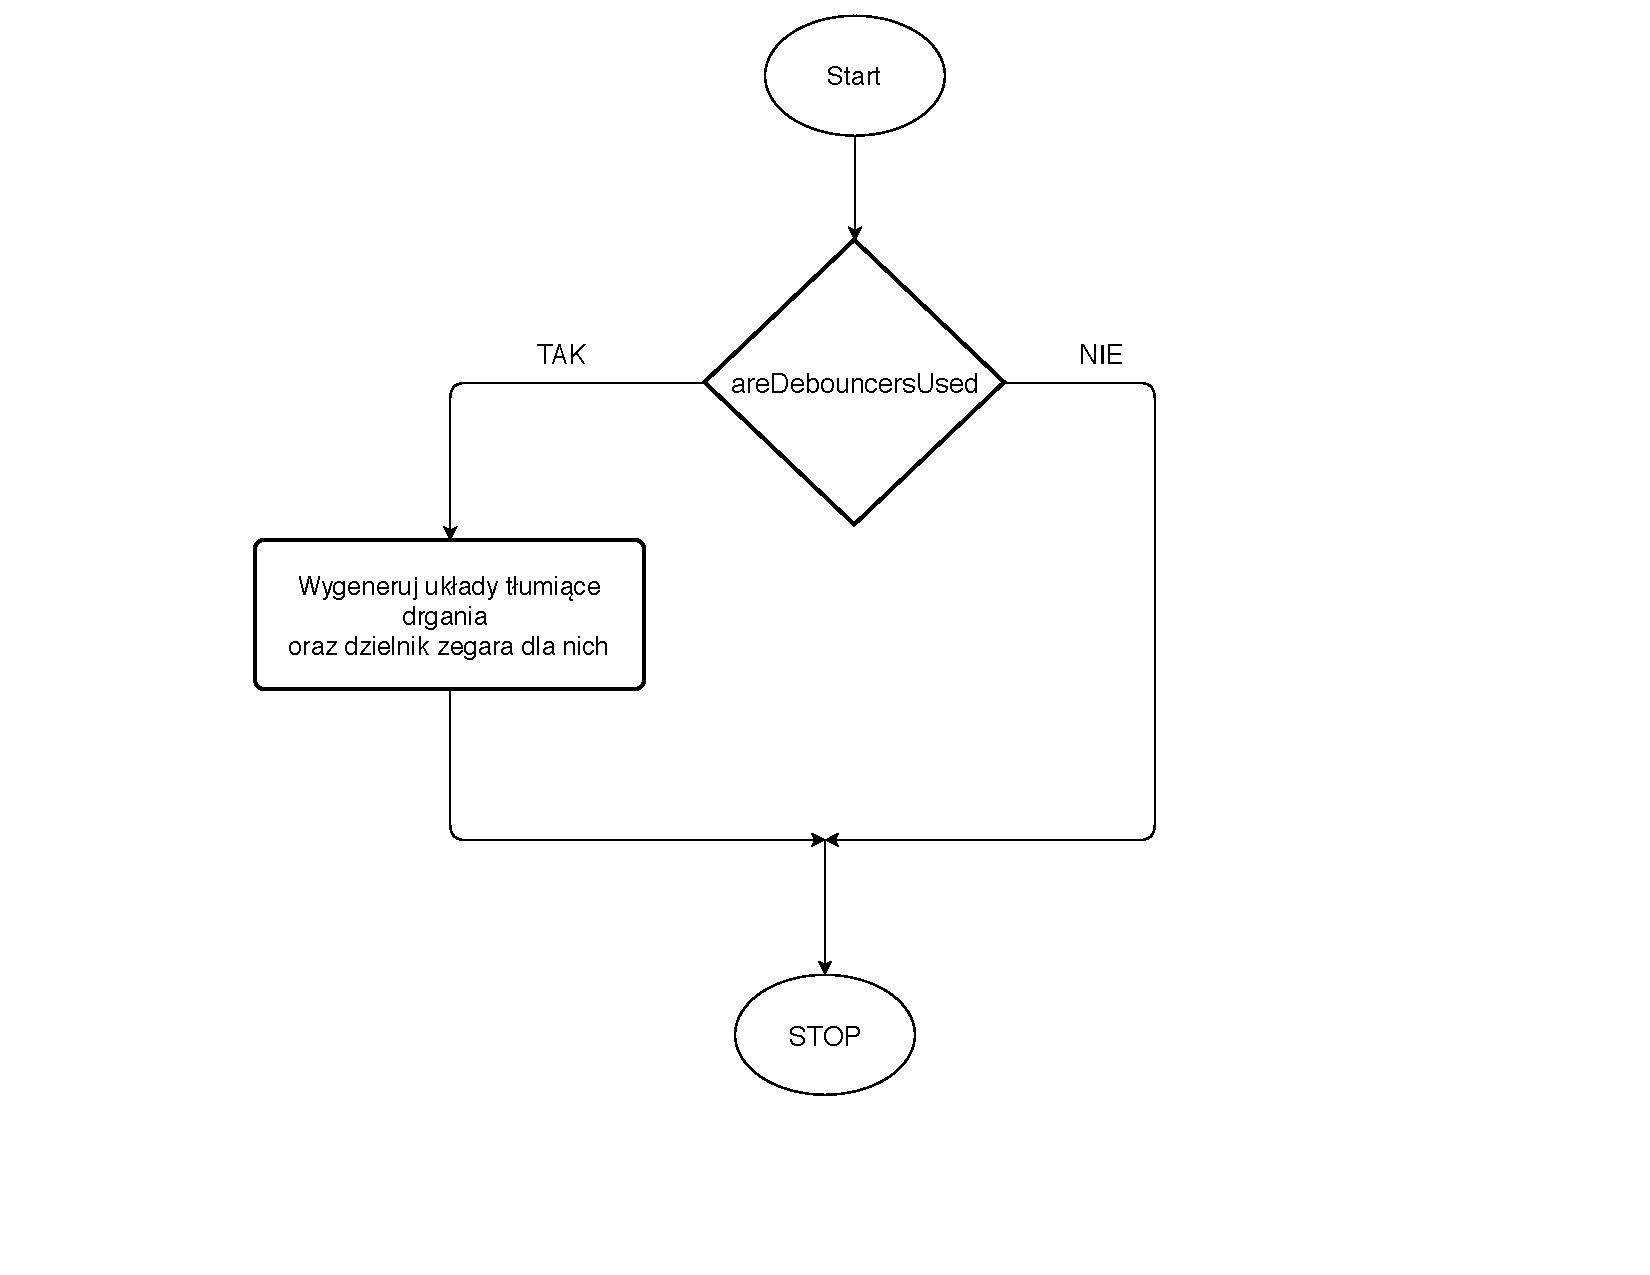
\includegraphics[width=\textwidth]{res/HDL_Generate.pdf}
\caption{Schemat blokowy - idea działania algorytmu generującego debouncery w module SafeTop}
\label{fig:deb}
\end{figure}

\subsubsection{Moduł Bcd2Decades}
Jest to moduł stanowiący licznik modulo 32 zwracający wartość w formacie BCD (Binary Coded Decimal) o dwóch dekadach. Założenie formatu BCD polega na kodowaniu binarnie każdej z cyfr reprezentacji dziesiętnej wejścia osobno, tzn. np. dla wejścia (w postaci dziesiętnej) 15 osobno zakodowana zostanie cyfra 1 (co daje wynik 0001) oraz osobno cyfra 5 (co daje wynik 0101). Ostatecznie otrzymujemy więc wynik 0001 0101. Moduł Bcd2Decades składa się ze zwykłego licznika binarnego modulo 32, przerzutnika wyjściowego oraz z procesu kombinacyjnego implementującego algorytm konwersji wartości binarnej na postać BCD. Zastosowano następujący algorytm konwersji:
\begin{enumerate}
\item Inicjalizujemy wartości kolumn (dziesiątki i jednostki) wartością zero.
\item Jeśli wartość w którejkolwiek z kolumn jest większa lub równa 5, dodajemy do niej wartość 3.
\item Wykonujemy przesunięcie bitowe o jeden w lewo, przy czym najstarszy bit jednostek staje się najmłodszym bitem dziesiątek i analogicznie najstarszy bit wartości binarnej staje się najmłodszym bitem jednostek - traktujemy je tak, jakby były ustawione w następujący sposób: \{dziesiątki, jednostki, wartość binarna\}
\item Jeśli przeprowadzono 5 iteracji (5 razy dokonano przesunięcia bitowego - liczba 5 to liczba bitów, za pomocą której reprezentujemy wartość binarną), to kończymy działanie. W przeciwnym razie powrót do kroku numer 2. 
\end{enumerate}
Implementacja algorytmu przestawiona została na listingu \ref{lst:bcd}. Przykładowy jego przebieg zawiera natomiast tabela \ref{table:bcdexample}.
\begin{lstlisting}[style={verilog-style}, caption={Implementacja algorytmu zamiany wartości binarnej na postać BCD.}, label={lst:bcd}]
reg [3:0] bcd0tmp;
reg [3:0] bcd1tmp;
always@* begin
    automatic integer i = 0;
    bcd0tmp = 4'b0000;
    bcd1tmp = 4'b0000;
    for (i = 0; i < 5; i = i + 1) begin
        bcd0tmp = (bcd0tmp >= 5 ? bcd0tmp + 4'd3 : bcd0tmp);
        bcd1tmp = (bcd1tmp >= 5 ? bcd1tmp + 4'd3 : bcd1tmp);
            
        bcd1tmp = bcd1tmp << 1;
        bcd1tmp[0] = bcd0tmp[3];
        bcd0tmp = bcd0tmp << 1;
        bcd0tmp[0] = binary_counter[bits-i-1];
    end
end
\end{lstlisting}

\begin{table}[H]
\centering
\caption{Prezentacja działania algorytmu konwersji wartości binarnej do postaci BCD na przykładzie liczby 17.}
\begin{tabular}{llll}
\toprule
\rowcolor[HTML]{ECF4FF} 
Dziesiątki                   & Jednostki                    & Postać binarna & Operacja                 \\ \midrule
0000                         & 0000                         & 10001          &                          \\
0000                         & 0001                         & 00010          & \textless{}\textless \#1 \\
0000                         & 0010                         & 00100          & \textless{}\textless \#2 \\
0000                         & 0100                         & 01000          & \textless{}\textless \#3 \\
0000                         & \cellcolor[HTML]{FFFFC7}1000 & 10000          & \textless{}\textless \#4 \\
0000                         & \cellcolor[HTML]{FFFFC7}1011 & 10000          & dodaj 3                  \\
\cellcolor[HTML]{9AFF99}0001 & \cellcolor[HTML]{9AFF99}0111 & 00000          & \textless{}\textless \#5 \\
\bottomrule  
\end{tabular}
\label{table:bcdexample}
\end{table}


\subsubsection{Moduł RseDecoder}
Moduł \textbf{RseDecoder} odpowiada za odpowiednie przetwarzanie sygnału dostarczonego przez enkoder obrotowy. Sygnał dostarczany jest wcześniej odpowiednio debounceowany w celu eliminacji drgań. Logika modułu opiera się na odpowiedniej maszynie stanów przedstawionej na Rysunku \ref{fig:rsedec}. Moduł sygnalizuje ruch rygla oraz jego kierunek osiągając stany \textit{clockwiseCounter} oraz \textit{counterClockwiseCounter}. Zmiana kierunku jest sygnalizowana poprzez przejścia z \textit{clockwisePosedge} na \textit{counterClockwiseCounter} oraz \textit{counterClockwisePosedge} na \textit{clockwiseCounter}.

\begin{figure}[H]
\centering
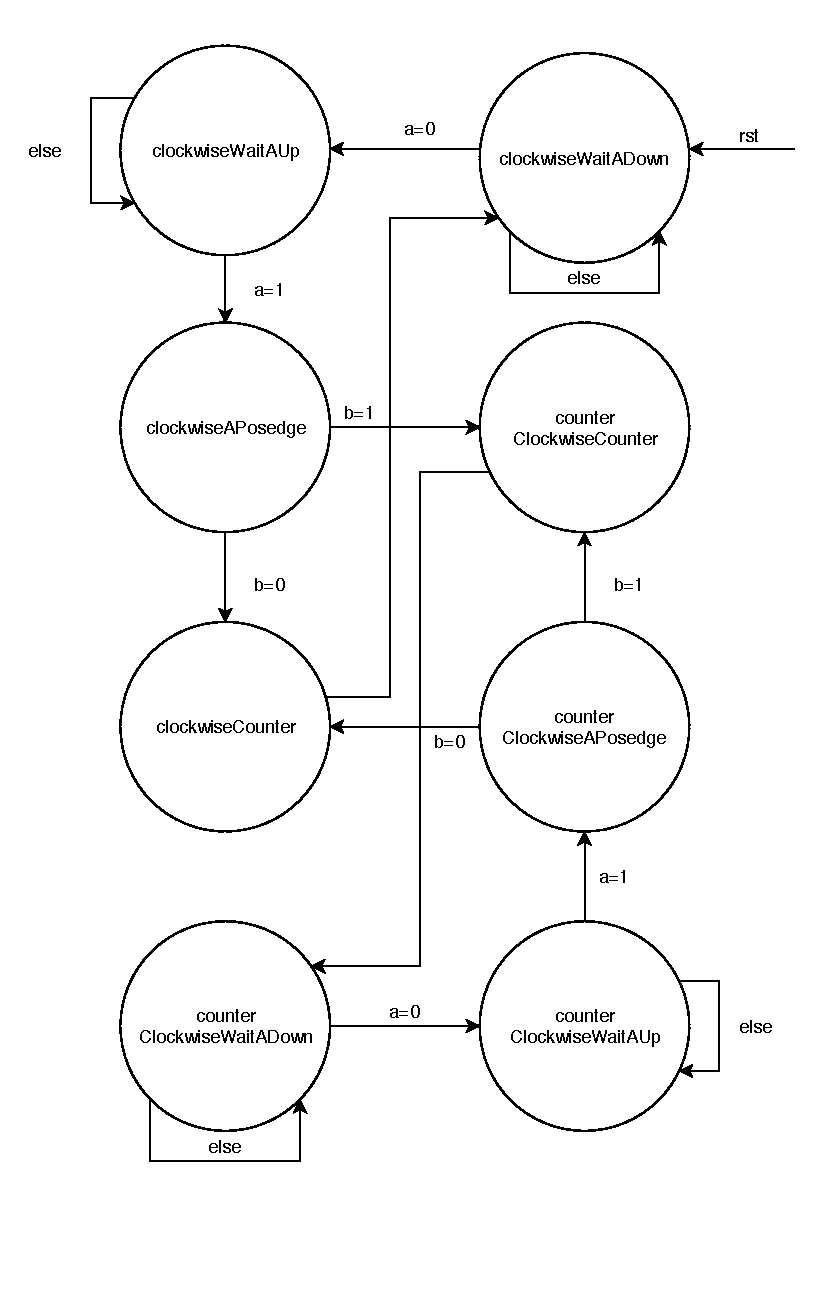
\includegraphics[width=0.9\textwidth]{res/rse_fsm_diagram.pdf}
\caption{Maszyna stanów RseDecoder}
\label{fig:rsedec}
\end{figure}

Wyjściami modułu są następujące sygnały:
\begin{itemize}
\item \textbf{knobCounterEnable} - sygnał informujący o odczycie obrotu
\item \textbf{isDirectionClockwise} - sygnał informujący czy odczytany obrót jest zgodny z kierunkiem wskazówek zegara (1) czy też nie (0)
\item \textbf{isDirectionChanged} - sygnał informujący o zmianie kierunku obracania względem wcześniej zarejestrowanego kierunku
\end{itemize}


\subsubsection{Moduł MasterFsm}
Moduł \textbf{MasterFsm} odpowiada za główną logikę urządzenia. Decyduje on o otwarciu sejfu. Głównym jego członem jest maszyna stanów, która jest przedstawiona na Rysunku \ref{fig:masterfsm}. Znajdują się w niej przejścia między stanami sprawdzania poprawności kolejnych części szyfru, otwarcia/zamknięcia sejfu. Poprawność szyfru jest sprawdzana w momencie zmiany kierunku sygnalizowanej przez \textbf{RseDecoder}, sprawdzenia dokonuje moduł \textbf{DigitCompare} zwracając informacje do \textbf{MasterFsm}. Przejścia w module \textbf{MasterFsm} zależą również od przycisków (sygnały open, lock) oraz od przełącznika (sygnał doorCls).

\begin{figure}[H]
\centering
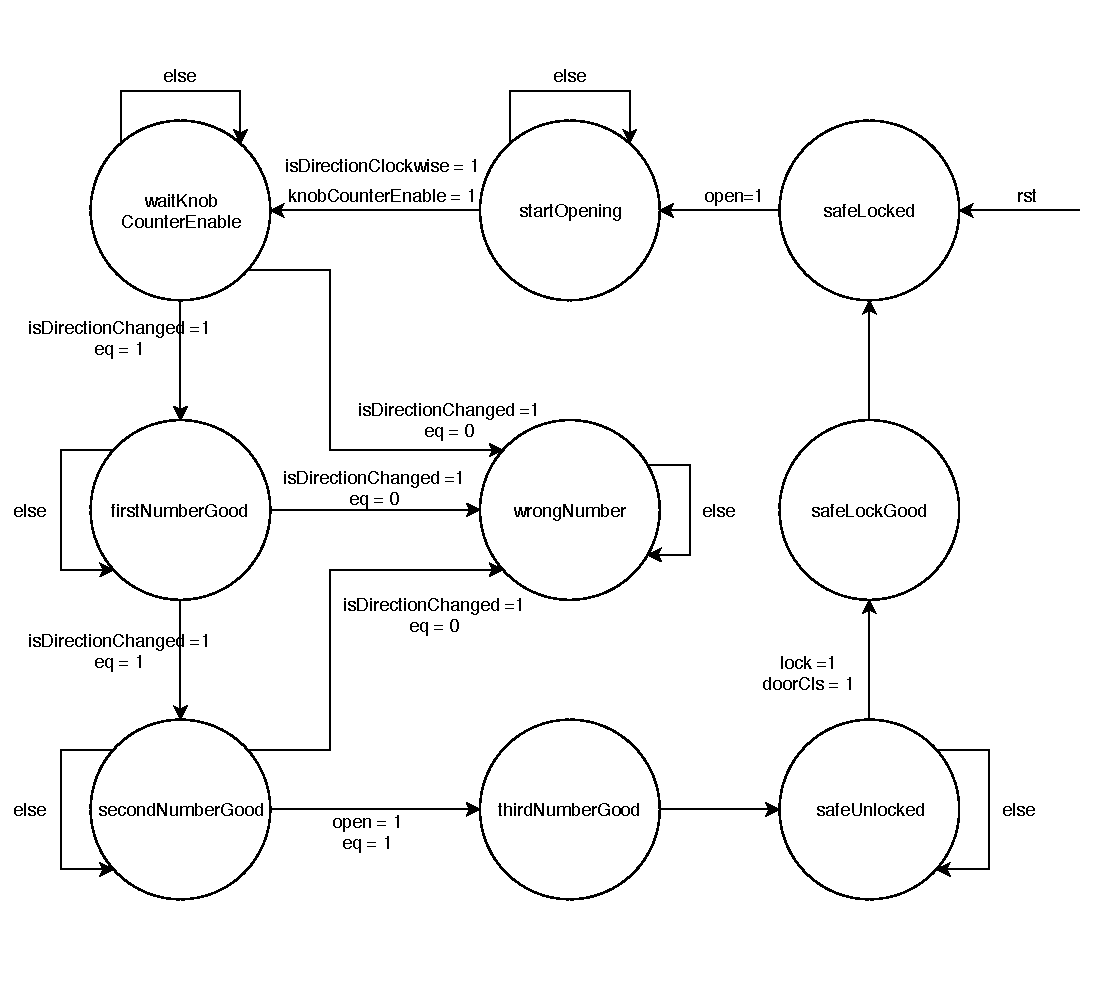
\includegraphics[width=0.9\textwidth]{res/master_fsm_diagram.pdf}
\caption{Maszyna stanów MasterFsm}
\label{fig:masterfsm}
\end{figure}

\newpage
Wyjściami modułu są sygnały:
\begin{itemize}
\item \textbf{enableCounter} - uruchomienie licznika
\item \textbf{clearCounter} - wyzerowanie licznika
\item \textbf{blank} - wyczyszczenie wyświetlacza
\item \textbf{triggerLock} - uruchomienie rygla
\item \textbf{isLockBeingOpened} - kierunek ruchu rygla (otwierający/zamykający)
\item \textbf{numberSelector} - wskazuje która liczba szyfru jest aktualnie obsługiwana
\end{itemize}

\newpage
\section{Analiza raportu syntezy}

Rozdział zawiera analizę raportu syntezy wygenerowanego przez narzędzie \textbf{Xilinx Vivado 2019.1}. Analizie poddane zostały:
\begin{itemize}
\item Sposób kodowania stanów
\item Użyte zasoby, np.: ROM, komórki logiczne
\end{itemize}

\subsection{Kodowanie stanów}
\begin{itemize}
\item W większości przypadków zastosowane zostało kodowanie typu \textbf{one-hot}, co jest zwykle zachowaniem domyślnym dla narzędzi Xilinx
\item Dotyczy to następujących modułów: MasterFsm, RseDecoder, Spi, FsmOper, FsmInit
\item Tabela \ref{table:onehot} przedstawia przykładowe kodowanie \textbf{one-hot}
\begin{table}[H]
\centering
\caption{Przykład kodowania typu one-hot zaistniały w wyniku syntezy projektu (moduł MasterFsm)}
\begin{tabular}{@{}lll@{}}\\
\toprule
\rowcolor[HTML]{DAE8FC} 
\textbf{Stan (State)} & \textbf{Nowe kodowanie} & \textbf{Poprzednie kodowanie}\\ \midrule
safeLocked            & 000000001                     & 00000000000000000000000000000000         \\
startOpening          & 000000010                     & 00000000000000000000000000000001         \\
waitKnobCounterEnable & 000000100                     & 00000000000000000000000000000010         \\
firstNumberGood       & 000001000                     & 00000000000000000000000000000011         \\
secondNumberGood      & 000010000                     & 00000000000000000000000000000100         \\
thirdNumberGood       & 000100000                     & 00000000000000000000000000000101         \\
safeUnlocked          & 001000000                     & 00000000000000000000000000000111         \\
safeLockGood          & 010000000                     & 00000000000000000000000000001000         \\
wrongNumber           & 100000000                     & 00000000000000000000000000000110         \\
\bottomrule    
\end{tabular}
\label{table:onehot}
\end{table}
\item W przypadku pozostałych maszyn stanów (Delay, UpdatePage, OledDriver) zostało zastosowane kodowanie sekwencyjne.
\item Tabela \ref{table:seq} przedstawia przykładowe kodowanie \textbf{sekwencyjne}:
\begin{table}[H]
\centering
\caption{Przykład kodowania typu sequential zaistniały w wyniku syntezy projektu (moduł UpdatePage)}
\begin{tabular}{@{}lll@{}} \\
\toprule
\rowcolor[HTML]{DAE8FC} 
\textbf{Stan (State)} & \textbf{Nowe kodowanie} & \textbf{Poprzednie kodowanie}    \\ \midrule
idle                  & 000                     & 00000000000000000000000000000000 \\
ClearDC               & 001                     & 00000000000000000000000000000001 \\
SendCmd               & 010                     & 00000000000000000000000000000010 \\
Transition1           & 011                     & 00000000000000000000000000000100 \\
Transition2           & 100                     & 00000000000000000000000000000101 \\
Transition5           & 101                     & 00000000000000000000000000000110 \\
SetDC                 & 110                     & 00000000000000000000000000000011 \\
\bottomrule  
\end{tabular}
\label{table:seq}
\end{table}
\end{itemize}

\subsection{Użycie zasobów}
\begin{itemize}
\item Użyty został jeden blok ROM o rozmiarach 1024x8. Przeznaczony on jest na przechowywanie informacji o czcionce - informacje wczytane z pliku \textbf{pixel\_SSD1306.dat}
\item Cały projekt składa się z \textbf{635} komórek logicznych (cells), w tym największą ilość stanowią komórki typu \textbf{FDCE} oraz \textbf{LUT} z różną ilością argumentów.
\item Tabela ~\ref{table:tabcells} przedstawia użycie komórek w poszczególnych modułach projektu.
\end{itemize}
\begin{table}[H]
\centering
\caption{Zużycie komórek logicznych przez poszczególne moduły projektu}
\begin{tabular}{@{}llll@{}}
\toprule
\rowcolor[HTML]{DAE8FC} 
\textbf{} & \textbf{Instancja}                     & \textbf{Moduł}             & \textbf{Komórki (Cells)} \\ \midrule
1         & top                                    &                            & 635                      \\
2         & - BCD2DEC                              & Bcd2Decades                & 30                       \\
3         & - CLK\_DIV                             & ClockDiv\_\_parameterized0 & 57                       \\
4         & - LED\_DRIVER                          & LedDriver                  & 2                        \\
5         & - MASTER\_FSM                          & MasterFsm                  & 37                       \\
6         & - OLED\_DRIVER                         & OledDriver                 & 375                      \\
7         & - - FSM\_INIT                          & FsmInit                    & 180                      \\
8         & - - - DELAY                            & Delay                      & 71                       \\
9         & - - - SPI                              & Spi\_2                     & 52                       \\
10        & - - FSM\_OPER                          & FsmOper                    & 184                      \\
11        & - - - CHAR\_LIB\_COM                   & Rom                        & 1                        \\
12        & - - - PAGE\_ROW                        & UpdatePage                 & 27                       \\
13        & - - - SPI                              & Spi                        & 47                       \\
14        & - RSE\_DECODER                         & RseDecoder                 & 23                       \\
15        & - \textbackslash{}debGen.ADEBOUNCER    & DebouncerKnob              & 6                        \\
16        & - \textbackslash{}debGen.BDEBOUNCER    & DebouncerKnob\_0           & 6                        \\
17        & - \textbackslash{}debGen.DEBCLKDIV     & ClockDiv                   & 64                       \\
18        & - \textbackslash{}debGen.LOCKDEBOUNCER & DebouncerButtons           & 6                        \\
19        & - \textbackslash{}debGen.OPENDEBOUNCER & DebouncerButtons\_1        & 6                        \\ \bottomrule
\end{tabular}
\label{table:tabcells}
\end{table}

\newpage
\section{Testy}
Ostatni rozdział poświęcony został procesowi testowania projektu - w tym przygotowanym modułom testowym.

\subsection{Moduły testujące}
Projekt zawiera \textbf{10} modułów testowych (tzw. moduły \textit{Testbench}). Umożliwiają one przeprowadzenie symulacji działania modułów projektu. Testy przeprowadzone zostały za pomocą dwóch typów symulacji:
\begin{itemize}
\item symulacja behawioralna (\textit{behavioural simulation})
\item symulacja po syntezie z uwzględnieniem parametrów czasowych (\textit{post-synthesis timing simulation})
\end{itemize}
Podstawowa struktura większości modułów \textit{Testbench} jest podobna - składają się one z:
\begin{itemize}
\item deklaracji parametrów wejściowych modułu (jeśli takie są)
\item deklaracji zmiennych stanowiących wejścia i wyjścia testowanego modułu oraz zmiennej odpowiadającej za \textit{Global System Reset - GSR}
\item instancji testowanego modułu (\textit{UUT - Unit Under Test})
\item generacji sygnałów wejściowych testowanego modułu (w tym zwykle sygnału zegara i resetu)
\end{itemize}
Listing \ref{lst:testy} ilustruje opisaną powyżej strukturę.

\begin{lstlisting}[style={verilog-style}, caption={Uproszczona struktura wykonanych modułów testujących}, label={lst:testy}]
module TbExample();
    
    // parametry    
    localparam mod = 3;    
    
    // wejscia
    reg clk, rst;
    reg in1;
    
    // wyjscia
    reg [3:0] out1; 
    
    // ...

    // GSR - Global System Reset
    wire gsr = glbl.GSR;

    // UUT - Unit Under Test
    ExampleModule #(.mod(mod)) EXAMPLE (
        .clk(clk), .rst(rst), .in1(in1), .out1(out1));

    // generacja sygnalow wejsciowych

    // zegar
    initial begin
        clk = 1'b0;
        @(negedge gsr);
        forever #5 clk = ~clk;
    end
    
    // reset
    initial begin
        rst = 1'b1;
        @(negedge gsr);
        #5 rst = 1'b0;
    end
    
    // in1
    initial begin 
        // kod generujacy wartosci sygnalu in1
    end
    
    // ...
    
endmodule
\end{lstlisting}
W dalszej części tego podrozdziału omówione zostaną poszczególne moduły testujące oraz wyniki przeprowadzonych symulacji behawioralnych. 

\subsubsection{Testy modułu SafeTop}
Test modułu SafeTop zakłada wyłączenie generacji debouncerów w module. Rysunek \ref{fig:behavSafeTop} przestawia wartości sygnałów uzyskane podczas testu.  Podczas testu wygenerowana została odpowiednia kombinacja sygnałów wejściowych \textit{a} i \textit{b} (sygnały pochodzące z pokrętła), by wprowadzić poprawny szyfr sejfu. Po wprowadzeniu ostatniej wartości oraz wygenerowaniu sygnału open wartość sygnału \textit{diodes} zmienia się na taką, która wskazuje, że sejf został otwarty. Zachowanie modułu jest więc zgodne z oczekiwanym.
\begin{figure}[H]
\centering
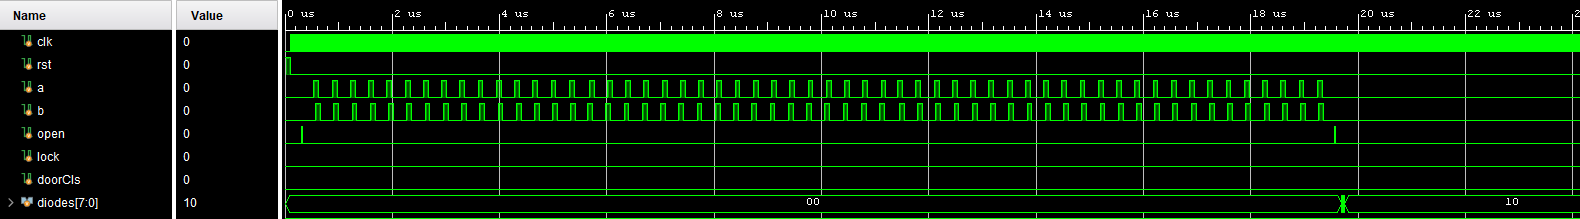
\includegraphics[width=\textwidth]{res/behav_sims/SafeTop_behavSim_1.png}
\caption{Wartości sygnałów wejściowych i wyjściowych podczas testu moduły SafeTop}
\label{fig:behavSafeTop}
\end{figure}

\subsubsection{Testy modułu Bcd2Decades}
Moduł Bcd2Decades odpowiedzialny jest za zliczanie sygnałów wejściowych oraz reprezentację licznika w postaci Binary Coded Decimal. Na każdym rosnącym zboczu zegara próbkowane są linie \textit{cnten1} oraz \textit{cnten2}. Jeśli na obu z nich występuje stan wysoki, to licznik jest modyfikowany zgodnie z kierunkiem wskazanym przez sygnał \textit{up}. Rysunek \ref{fig:behavBcd2Dec1} przedstawia pomyślnie przeprowadzony test opisanej funkcjonalności. Możliwe jest również wyzerowanie licznika za pomocą sygnału \textit{clrCount} - dokładnie takie działanie można zaobserwować na rysunku \ref{fig:behavBcd2Dec2}.


\begin{figure}[H]
\centering
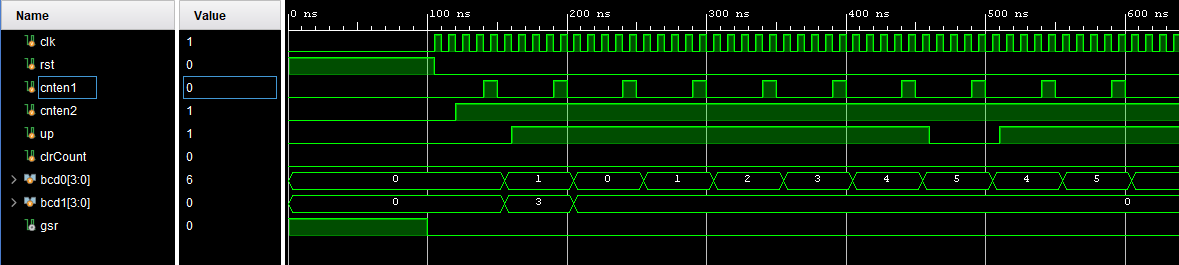
\includegraphics[width=\textwidth]{res/behav_sims/Bcd2Dec_behavSim_1.png}
\caption{Wartości sygnałów wejściowych i wyjściowych podczas testu moduły Bcd2Decades}
\label{fig:behavBcd2Dec1}
\end{figure}

\begin{figure}[H]
\centering
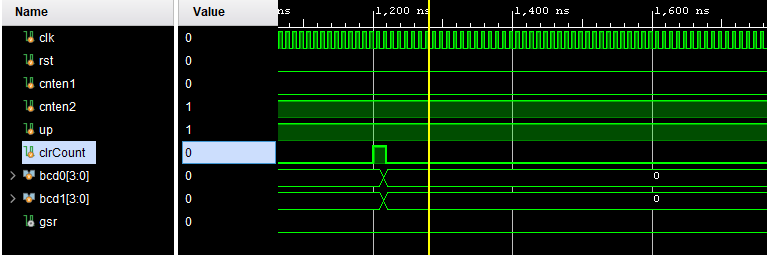
\includegraphics[width=\textwidth]{res/behav_sims/Bcd2Dec_behavSim_2.png}
\caption{Reakcja modułu Bcd2Decades na stan wysoki sygnału clrCount.}
\label{fig:behavBcd2Dec2}
\end{figure}





\subsubsection{Testy modułu RseDecoder}

Test moduły \textbf{RseDecoder} polega na wygenerowaniu sygnałów a i b o odpowiedniej długości oraz kolejności. Są one generowane w taki sposób, aby sygnalizować dwa razy ruch zgodny z kierunkiem wskazówek zegara, dwa razy ruch przeciwny do kierunku wskazówek zegara oraz dwa razy ruch zgodny z kierunkiem wskazówek zegara. Moduł testowy ukazany na Rysunku \ref{fig:rseDecTB} wykazuje, że \textbf{RseDecoder} poprawnie generuje sygnały wyjściowe dla zadanych sygnałów wejściowych.

\begin{figure}[H]
\centering
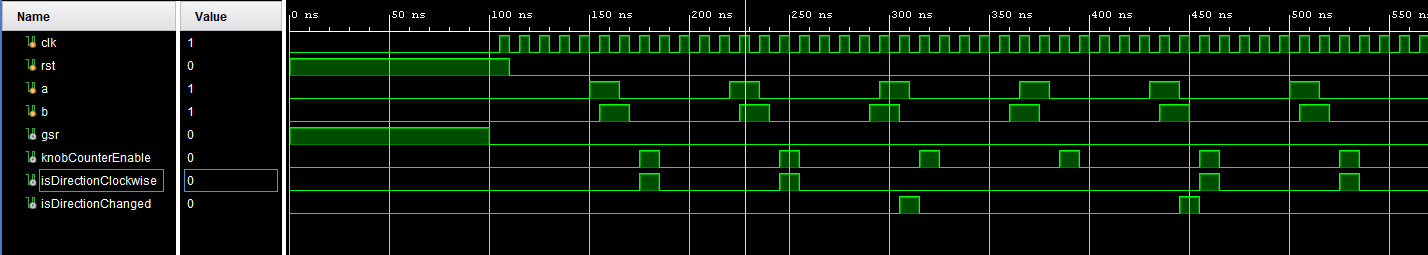
\includegraphics[width=\textwidth]{res/behav_sims/RseDecoder_behavSim_1.png}
\caption{Moduł testowy dla RseDecoder}
\label{fig:rseDecTB}
\end{figure}

\subsubsection{Testy modułu MasterFsm}
Test modułu \textbf{MasterFsm} polega na zaaplikowaniu odpowiednich sygnałów wejściowych, tak, aby maszyna stanów przeszła przez cały proces dla odpowiedniego otwierania sejfu. Zgodnie z Rysunkiem \ref{fig:masterFsmTb} moduł poprawnie reaguje na wszystkie sygnały na co wskazują m.in. stany przyjmowane przez moduł. 


\begin{figure}[H]
\centering
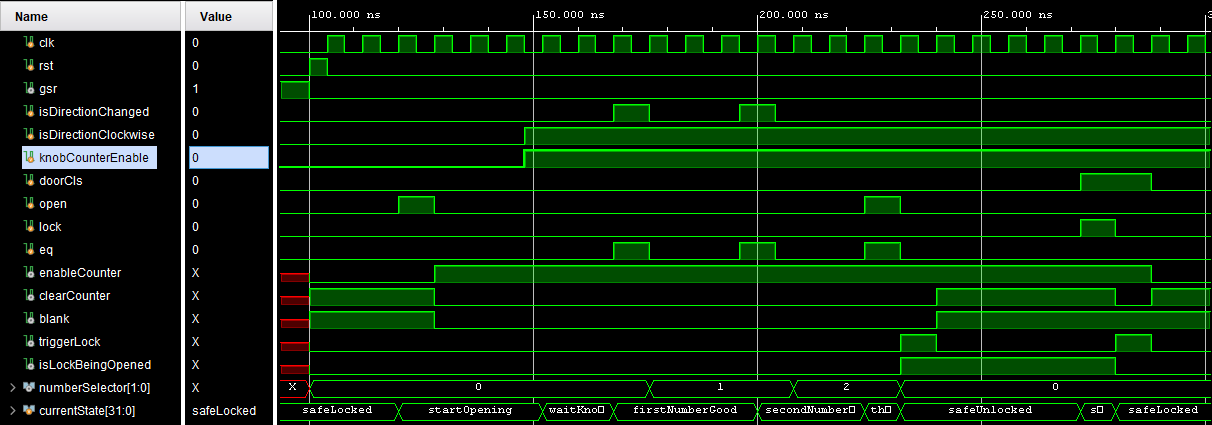
\includegraphics[width=\textwidth]{res/behav_sims/master_fsm_tb.png}
\caption{Moduł testowy dla MasterFsm}
\label{fig:masterFsmTb}
\end{figure}

\subsubsection{Testy modułu ClockDiv}
Test modułu ClockDiv jest bardzo prosty. Jego rezultaty przedstawione zostały na rysunku \ref{fig:behavClockDiv}. Na wejście modułu podawany jest zegar. Długość okresu wynikowego zegara (\textit{slowClk}) ustalona została za pomocą parametru na sześć okresów zegara wejściowego. Test wskazuje więc, że działanie modułu jest zgodne z oczekiwaniami - okres sygnału \textit{slowClk} jest sześć razy dłuższy od okresu sygnału \textit{clk}.

\begin{figure}[H]
\centering
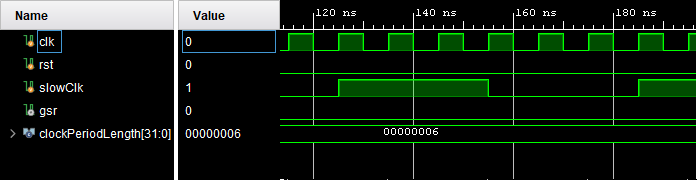
\includegraphics[width=\textwidth]{res/behav_sims/ClkDiv_behavSim_1.png}
\caption{Wartości sygnałów wejściowych i wyjściowych podczas testu moduły ClockDiv}
\label{fig:behavClockDiv}
\end{figure}


\subsubsection{Testy modułu DebouncerButtons}
Rysunek \ref{fig:behavDebounderButtons} przedstawia przebieg symulacji modułu DebouncerButtons. Moduł ten próbkuje na każdym rosnącym zboczu zegara wartość na linii \textit{in}. Jeśli w ciągu 3 kolejnych próbek linia utrzymuje stan wysoki, na wyjściu \textit{out} generowany jest sygnał o wartości 1. Obserwacja przebiegów pozwala stwierdzić, że moduł zachowuje się zgodnie z oczekiwaniami.

\begin{figure}[H]
\centering
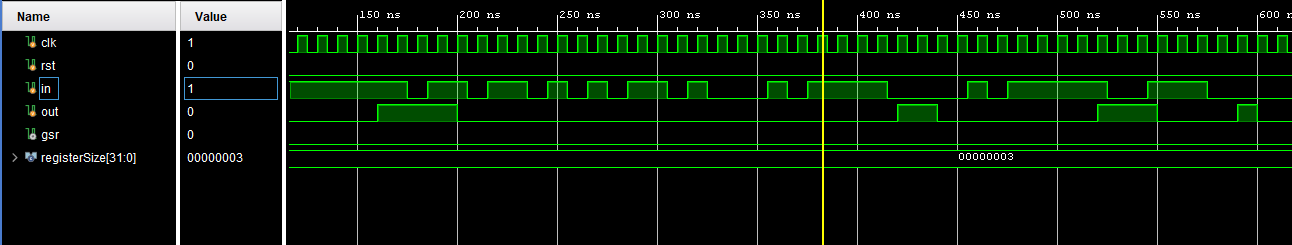
\includegraphics[width=\textwidth]{res/behav_sims/DebouncerButtons_behavSim_1.png}
\caption{Wartości sygnałów wejściowych i wyjściowych podczas testu moduły DebouncerButtons}
\label{fig:behavDebounderButtons}
\end{figure}




\subsubsection{Testy modułu DigitCompare}
Test modułu DigitCompare polegał na podawaniu na wejście modułu różnych możliwych wartości szyfru i porównywaniu ich z prawdziwym szyfrem (tutaj 15, 30, 22). W momencie, gdy podana na wejście liczba (w postaci BCD - sygnał \textit{bcd1} to cyfra dziesiątek, a \textit{bcd0} to jedności) jest zgodna z aktualnie sprawdzaną wartością szyfru, sygnał \textit{eq} powinien zmienić swój stan na wysoki. Rysunek \ref{fig:behavDigitCompare} przedstawia przebieg testu. Wynik symulacji wskazuje na poprawne działanie modułu.

\begin{figure}[H]
\centering
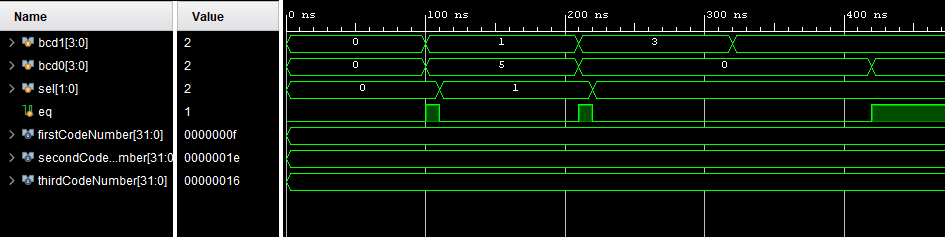
\includegraphics[width=\textwidth]{res/behav_sims/DigitCompare_behavSim_1.png}
\caption{Wartości sygnałów wejściowych i wyjściowych podczas testu moduły DigitCompare}
\label{fig:behavDigitCompare}
\end{figure}

\subsubsection{Testy modułu OledDriver}
Moduł OledDriver reaguje na zmianę wartości sygnału \textit{blank} oraz wektora \textit{bcdData}. Test polegał więc na odczekaniu, aż zakończy się proces inicjalizacji wyświetlacza OLED, a następnie na zmianie jednego z tych dwóch sygnałów. W momencie zmiany przewidywanym zachowaniem jest nastąpienie transmisji SPI, co powinno być widoczne na linii \textit{sdo}. Przebieg symulacji (rysunek \ref{fig:behavOledDriver}) potwierdza przewidywania - moduł działa poprawnie.

\begin{figure}[H]
\centering
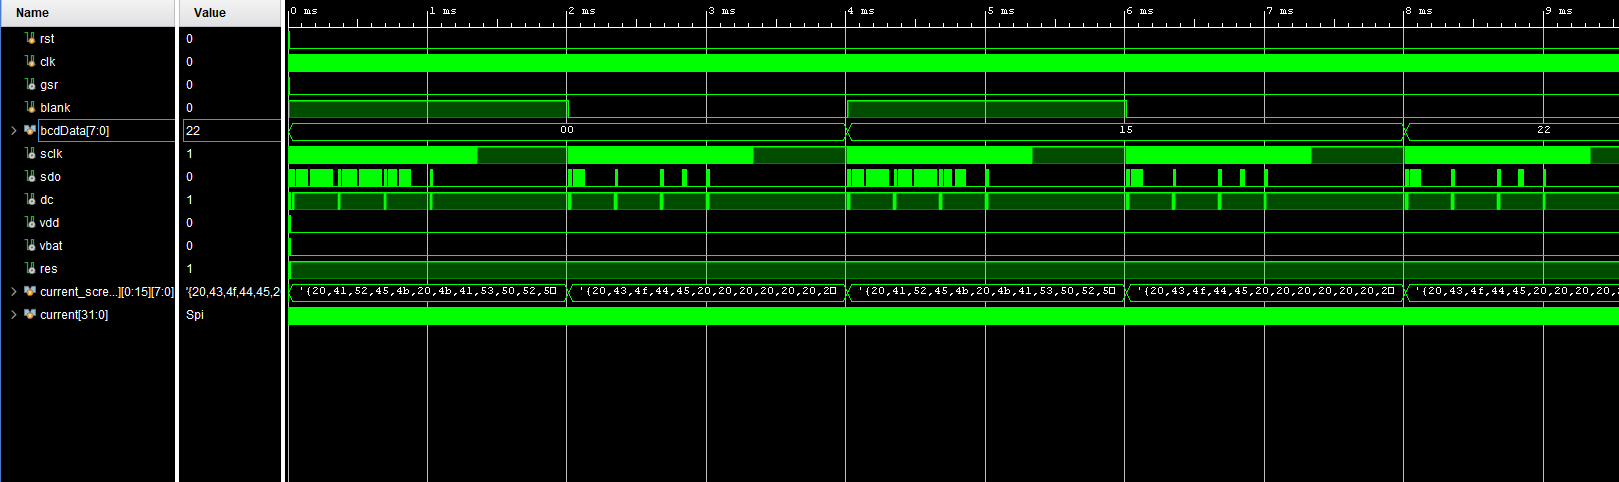
\includegraphics[width=\textwidth]{res/behav_sims/OledDriver_behavSim_1.png}
\caption{Wartości sygnałów wejściowych i wyjściowych podczas testu moduły OledDriver}
\label{fig:behavOledDriver}
\end{figure}


\subsubsection{Testy modułu Delay}
Na potrzeby testu moduł Delay został skonfigurowany za pomocą parametrów w taki sposób, by odliczał jedną milisekundę jako dziesięć okresów zegara (licznik \textit{cnt1ms)}. Po zakończeniu odliczania powinna wystąpić zmiana wartości sygnału \textit{fin} na stan wysoki. Ilość milisekund, które powinny zostać policzone (licznik \textit{cnt\_ms}) określa wartość sygnału wektora wejściowego \textit{delayLength}. Przebieg symulacji przedstawiony został na rysunku \ref{fig:behavDelay} - jest on zgodny z oczekiwaniami.

\begin{figure}[H]
\centering
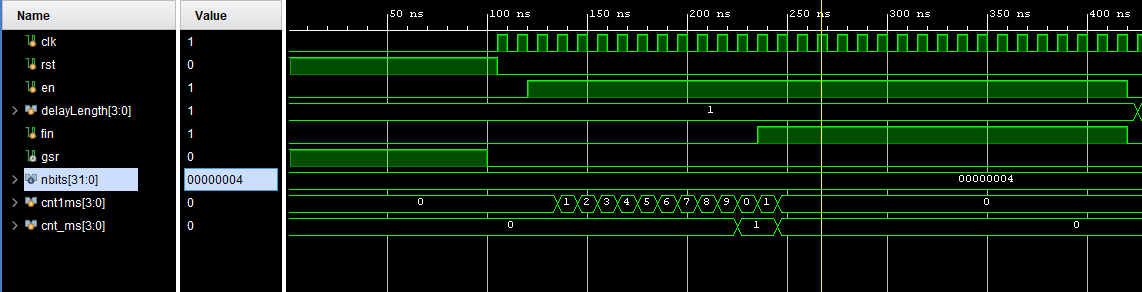
\includegraphics[width=\textwidth]{res/behav_sims/Delay_behavSim_1.png}
\caption{Wartości sygnałów wejściowych i wyjściowych podczas testu moduły Delay}
\label{fig:behavDelay}
\end{figure}


\section{Możliwe udoskonalenia}
Projekt niepozbawiony jest niedoskonałości. Najważniejsze z nich to:
\begin{itemize}
\item sporadyczny zły odczyt kierunku obracania pokrętła - skutkuje to zwykle wprowadzeniem niepoprawnego kodu i koniecznością powtórzenia procedury
\item przesuwanie się zawartości wyświetlacza OLED przy zmianie wyświetlanych danych
\end{itemize}


\newpage
\begin{thebibliography}{9}

\bibitem{skoczenagh} 
dr inż. Andrzej Skoczeń: materiały do przedmiotu Języki Opisu Sprzętu
\\\texttt{http://www.fis.agh.edu.pl/~skoczen/hdl/}

\bibitem{bcd1} 
Prezentacja Binary-to-BCD Converter dostępna na stronie:
\\\texttt{http://www.tkt.cs.tut.fi/kurssit/1426/S12/Ex/ex4/Binary2BCD.pdf}

\bibitem{bcd2} 
Opracowanie algorytmu konwersji wartości binarnych od BCD ze strony:
\\\texttt{https://my.eng.utah.edu/~nmcdonal/Tutorials/BCDTutorial/BCDConversion.html}


\end{thebibliography}

\end{document}
